\printbibliography[title=참고문헌]

\AppendixTitleToToc
\AttachAppendixTitleToSecnum

\appendix
\appendixpage*

%\chapterstyle{appendixdefault}
%\pagestyle{hangul}

\section{Github Codespace에서 ihaskell-notebook 실행하기}
\label{sec:codespace}

\subsection{교재 홈페이지 접속 및 코드스페이스 생성}
\begin{center}
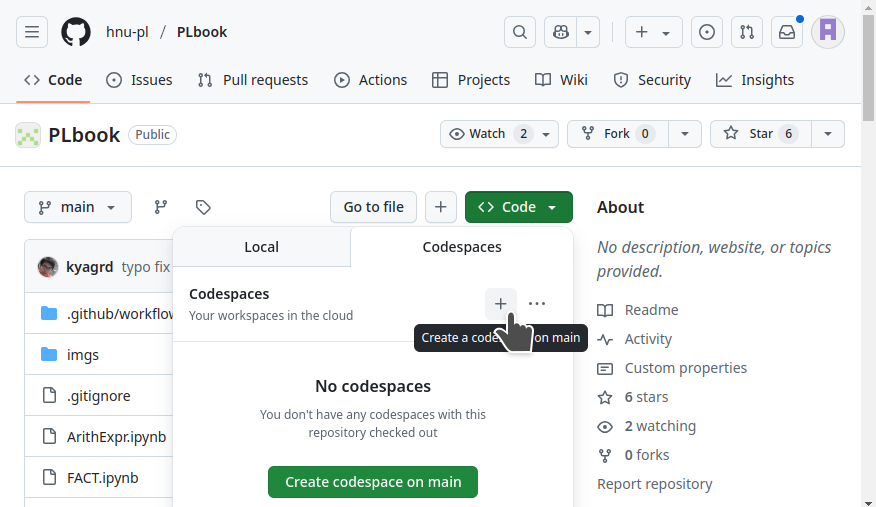
\includegraphics{GithubCodespace1.png}
\end{center}
위 캡춰 화면과 같이 Github에 로그인된 상태로 교재 홈페이지 접속 후,
녹색 Code 버튼을 클릭하고 Codespaces 탭을 선택하면 나타나는
`+'버튼을 Ctrl-클릭하여 새 탭에서 코드스페이스를 생성한다.
이 때, 코드스페이스 생성을 위한 환경설정 과정에 약간의 시간이 걸릴 수 있다.
이렇게 한번 생성한 이후에는, 같은 탭에서 ``No codespaces''의 위치에
이미 생성된 코드스페이스의 이름이 나타날 것이므로,
이를 Ctrl-클릭하여 활용하면 된다.

\begin{center}
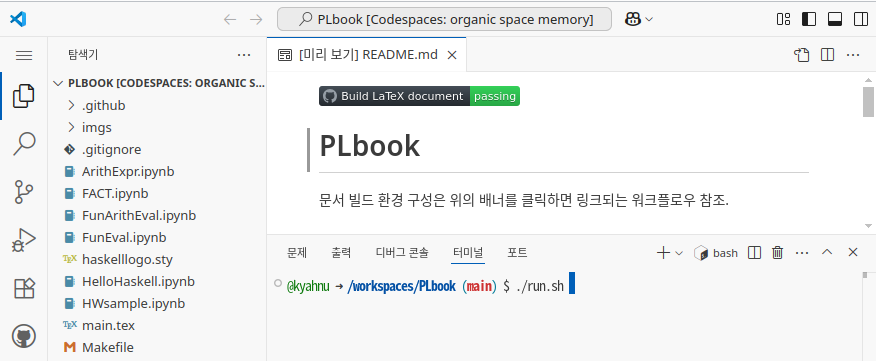
\includegraphics{GithubCodespace2.png}
\end{center}
코드스페이스가 성공적으로 생성되면 리눅스 명령어를 입력할 수 있는
터미널 패널이 나타나는데, 여기에서 앞의 캡춰 화면처럼
\texttt{run.sh} 스크립트로 주피터 서버를 실행한다.

\subsection{Jupyter 서버 실행 후 브라우저에서 열기}
\begin{center}
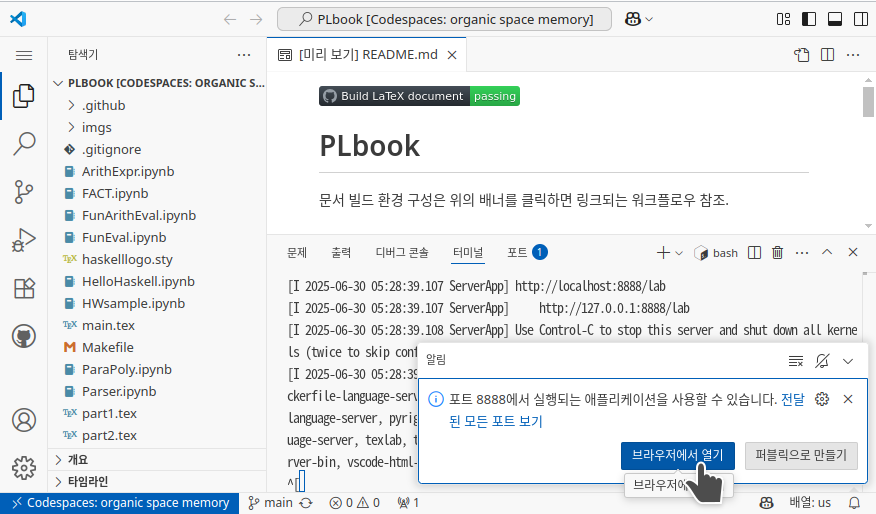
\includegraphics{GithubCodespace3.png}
\end{center}
주피터 서버가 실행되면 뜨는 팝업 알림에서 ``브라우저에서 열기''를 클릭하여
주피터 노트북에 접근할 수 있다. 팝업 알림을 실수로 닫았더라도
 `포트' 탭에서 자오선 지구본 모양을 클릭해 주피터 노트북에 접근할 수 있다.
\begin{center}
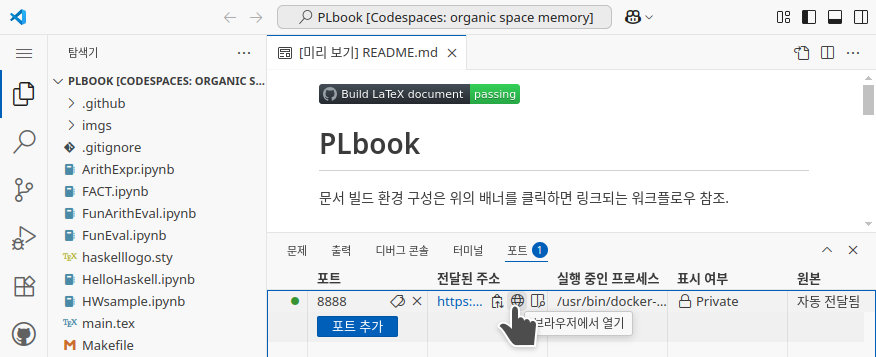
\includegraphics{GithubCodespace4.png}
\end{center}

\newpage

\section{과제 형식 예시}
\input{HWsample}

\newpage

\section{감사}
강의 노트를 교재의 형태로 이렇게 출간할 수 있게 된 데는 제가 컴퓨터과학을 전공하면서
인연을 맺게 된 은사님들과 정보과학회 프로그래밍언어연구회의 모든 분들에게 마땅히 감사한 마음이 있습니다.
하지만 여기에서 감사의 말씀을 표하기에는 너무 길어지는 관계로,
우선 이 책의 출간 과정에 직접적인 도움을 주신 출판사 관계자 분들,
수업 중에 오탈자를 보고해 준 수강생들, 그리고 프로그래밍언어론 과목에서
대학원생 조교로 수업 운영을 도우며 출판사를 섭외하는 등 다방면으로
신경써 준 제자인 손범준에게 이 지면을 빌어 간단히나마 감사의 기록을 남깁니다.

\subsection{초판 원고 작업본 오탈자 보고}
\subsubsection{2022년 1학기 프로그래밍언어론 수강생}
구준한, 권준호, 권혁준, 김동하, 김상운, 김이레, 김현, 백성욱, 백창현, 손현승,
신현수, 이승민, 이상빈, 장주안, 임영준, 장태영, 전석원, 정윤정, 정재훈, 황인규.

\subsubsection{2023년 1학기 프로그래밍언어론 수강생}
김민식, 김종윤, 박준형, 서지웅, 신수민, 윤승준, 이동복, 이재혁, 임도은, 정종운.

\subsubsection{2024년 1학기 프로그래밍언어론 수강생}
김지민, 문해찬, 명현철, 성재빈, 성준모, 장민혁, 유진호, 이강준, 이규호, 이승현, 이정아, 최태규, 한성준.

\begin{comment}
\newpage

\section{다음 판에 추가할지 고려중인 주제}
\subsection{Control}
Continuation-Passing Style,
Delimited Continuations,
Coroutines, Exceptions, Async-Await,
Algebraic Effects,
Functor/Applicative/Monad/Monoid/...

\url{https://www.microsoft.com/en-us/research/wp-content/uploads/2016/08/algeff-tr-2016-v2.pdf}

\subsection{Staged Computation}
Interpreter vs. Compiler, Futamura Projections, Partial Evaluation

\end{comment}


